\section{Prototype Implementation}
\label{sect:architecture}

Our prototype system runs on a cluster of Linux machines with Xen-based VMs 
and the QFS~\cite{michael2013} distributed file system. 
%to %manage  the physical disk storage. 
All data needed for the backup service including snapshot data and metadata
%and snapshot data for backup purposes, 
resides in this distributed file system. 
One physical node hosts tens of VMs, each of which accesses its virtual machine disk image through the
virtual block device driver (called TapDisk\cite{Warfield2005} in Xen).

\subsection{Per Node Software Components} 
%\begin{figure}[htbp]
\begin{figure}[htbp]
%\vspace{1em}
    \centering
    %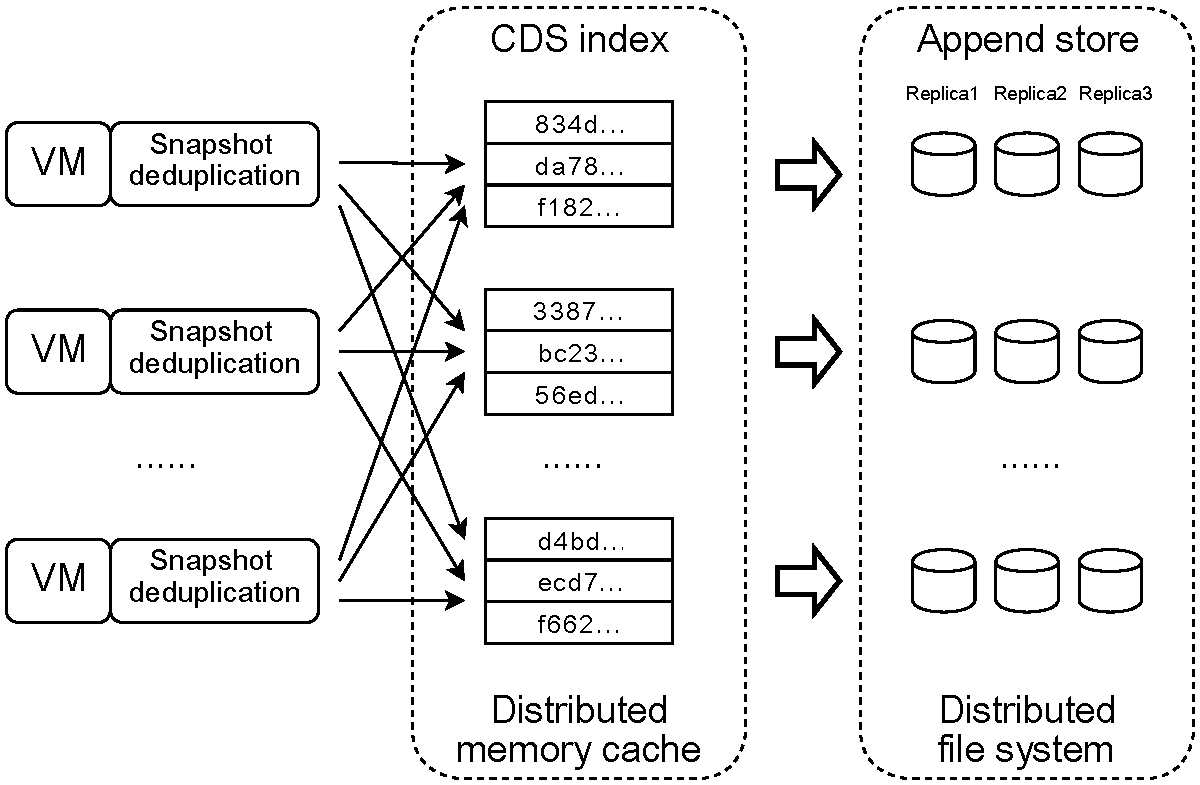
\includegraphics[width=2.75in]{images/socc_arch_cluster}
    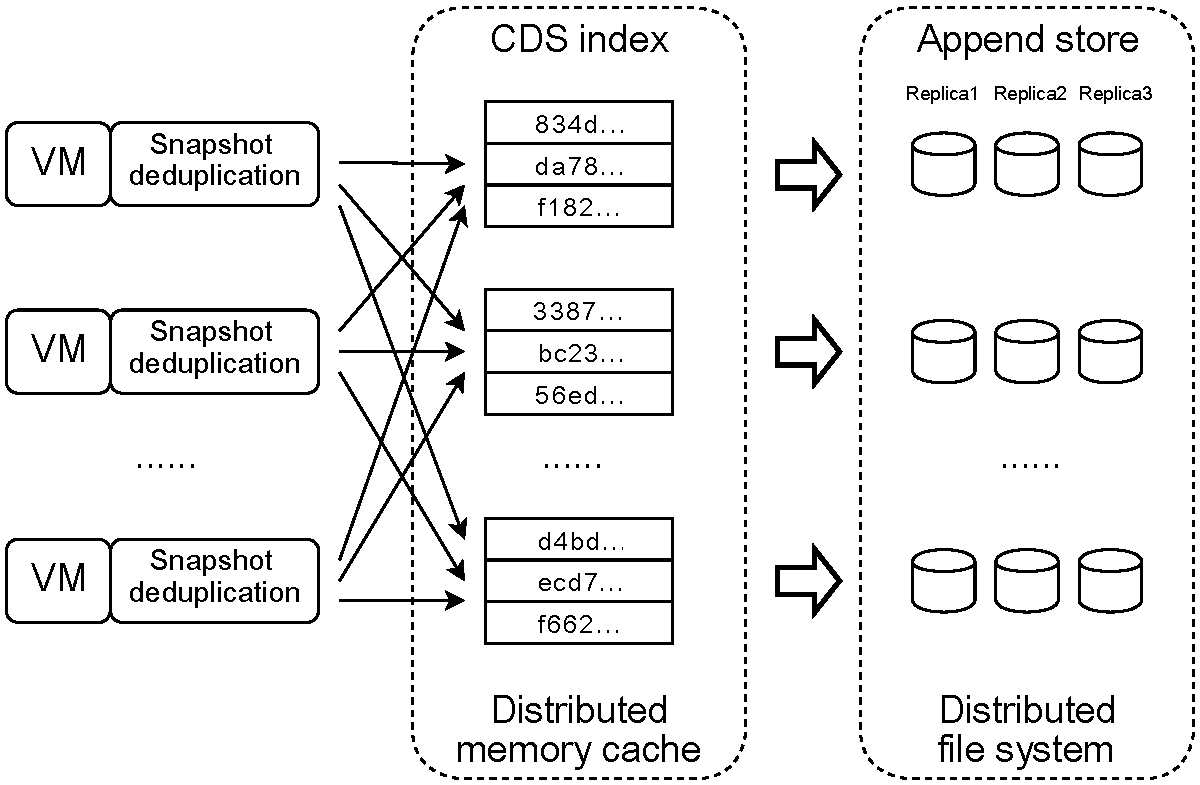
\includegraphics[width=3in]{images/socc_arch_cluster}
%\vspace{1em}
    \caption{Data flow during snapshot backup}
    \label{fig:arch_vm}
\end{figure}
As depicted in Figure~\ref{fig:arch_vm}, 
there are four key service components running on each cluster
node  for supporting backup and deduplication: 
1) a virtual block device driver, 2) a snapshot deduplication agent,
3) a snapshot store client to store  and access snapshot data,
and 4)  a PDS client to support PDS metadata access. 

We use the virtual device driver in Xen that employs a bitmap to track the changes 
that have been made to the virtual disk.
Every bit in the bitmap represents a fixed-sized (2MB) segment, indicating whether the segment
has been modified since last backup. 
Segments are further divided into variable-sized chunks (average 4KB) 
using a content-based chunking algorithm~\cite{frame05}, 
which brings the opportunity of fine-grained deduplication.
When the VM issues a disk write, the dirty bit for the corresponding segment is set
and this indicates such a segments needs to be checked during snapshot backup. 
After the snapshot backup is finished, the driver resets the dirty bit map to a clean state.
For data modification during backup, copy-on-write protection is set so that backup can continue to
copy  a specific version while new changes are recorded.
%copies a frozen version while the modification can still carry on.

The representation of each snapshot has  a two-level index data structure.
The snapshot meta data (called snapshot recipe) contains a list of segments, each of which contains segment
metadata of its chunks (called segment recipe).
In snapshot and segment recipes, 
the data structures  include references to the actual data location to eliminate the need for additional indirection.


\subsection{A VM-centric Snapshot Store}
\label{sect:store}

%\begin{figure}[htbp]
\begin{figure}[htbp]
%\vspace{1em}
  \centering
%  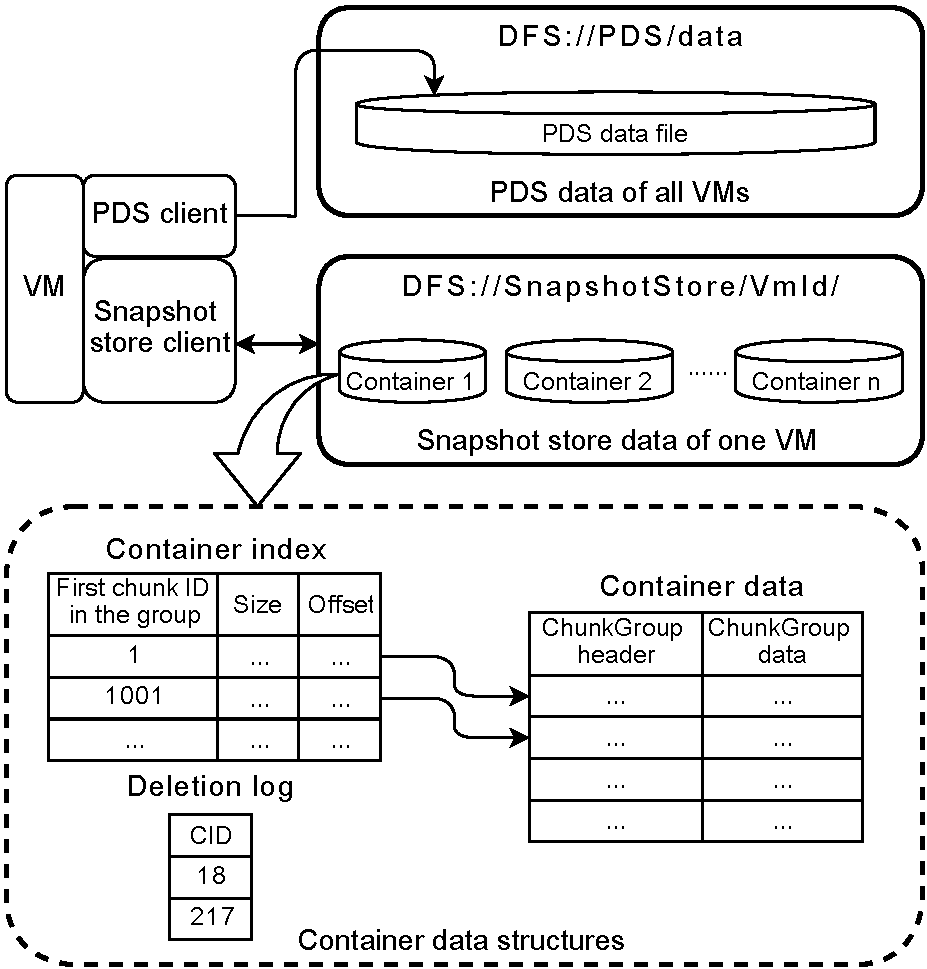
\includegraphics[width=2.75in]{images/sstore_arch}
  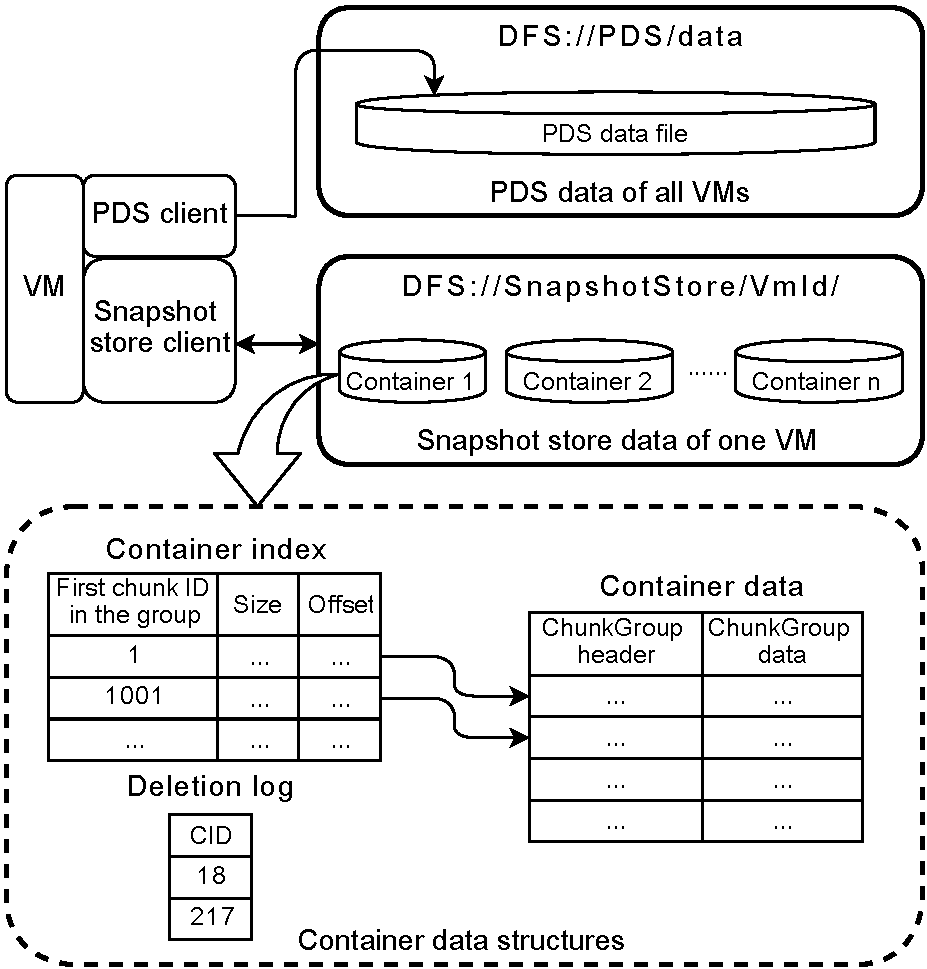
\includegraphics[width=3in]{images/sstore_arch}
%\vspace{1em}
  \centering
  \caption{VM snapshot store data structures}
  \label{fig:as_arch}
\end{figure}

We use the QFS distributed file system to hold snapshot backups.
Following the VM-centric idea for the purpose of fault isolation,
each VM has its own snapshot store, containing new data chunks which are considered
to be non-duplicates.
As shown in Figure~\ref{fig:as_arch}, we explain the data structure of the snapshot stores as follows.
%\begin{itemize}
%\item
There is an independent store containing all PDS chunks shared among different VMs as
a single file.
%All PDS chunks are stored in one PDS file. 
Each reference to a PDS data chunk in the PDS index is the offset within the PDS file.
%There is an option to use a data structure similar to the non-PDS store. We opt
%for the simpler format because
Additional compression is not applied because 
for the data sets we have tested, we only observed limited spatial locality 
among popular data chunks. On average the number of consecutive PDS index hits is lower than 7,
thus it is not very effective to group a large number of chunks as a compression and data fetch unit. 
For the same reason, we decide not to take the sampled index approach~\cite{Guo2011} 
for detecting duplicates from PDS as limited spatial locality is not sufficient to enable
effective prefetching for sampled indexing.

PDS data are re-calculated periodically in an offline manner, but 
the total data size is small.  When
a new PDS data  set is computed, the in-memory PDS index is replaced, but 
the PDS file on the disk appends the  new PDS data identified and the growth of this file is very slow. 
The old data are not removed because they can still be referenced by the existing snapshots. 
A periodic cleanup is conducted  to remove unused PDS chunks (e.g. every few months). 

%\end{itemize}

For non PDS data, the snapshot store of a VM is  divided into a set of containers and 
each container is approximately 1GB.  The reason for this  divison is to simplify the compaction process
conducted periodically. When  chunks are deleted from old snapshots,
chunks without any reference from other snapshots can be removed by this compaction process.
By limiting the size of a container, we can control the length of each round of compaction.
The compaction  can work on one container at a time and move the in-use data chunks to another container. 

Each non-PDS data container is further divided into a set of chunk data groups. Each chunk group is composed of
a set of data chunks and is the basic unit in data access and retrieval. 
In writing a chunk during backup, the system accumulates data chunks and stores the entire
group as a unit after compression. This  compression can reduce data by several times  in our tested data.
When accessing a particular chunk, its chunk group is retrieved from the storage
and decompressed. Given the high spatial locality and usefulness of prefetching  in 
snapshot chunk accessing~\cite{Guo2011,Rhea2008},
retrieval of  a data chunk  group naturally works well with prefetching. 
A  typical chunk group contains 1000 chunks in our experiment.
% with an average size of 200-600 chunks.

%\item
Each non-PDS data container is represented by three files in the DFS:
1) the container data file holds the actual content, 
2) the container index file is responsible for translating a data reference
into its location within a container, and 
3) a chunk deletion log file records all the deletion requests within  the container.

%\item
A non-PDS data chunk reference stored in the index of snapshot recipes
is composed of two parts: a container ID with 2 bytes and a local chunk ID with 6 bytes.
Each container maintains a local  chunk counter and assigns the current number 
as a chunk ID  when  a new chunk is added to this  container. 
Since data chunks are always appended to a snapshot store during backup, 
local chunk IDs are monotonically increasing.
When a chunk is to be accessed, the segment recipe contains a reference pointing to  a data chunk, which is used to lookup up the chunk data as described shortly.

%\item


Three API calls are supported for data backup:
\begin{itemize}

\item
\noindent\textbf{Append()}. 
For PDS data, the chunk is appended to the end of the PDS file and the offset is returned as the  reference.
This operation  may only be used during PDS recalculation.
For non-PDS data, this call places a chunk into 
the snapshot store and returns a reference to be stored in the recipe of a snapshot. 
The write requests to append chunks to a VM store are accumulated at the client side. 
When the number of write requests reaches a fixed group size, the client compresses
the accumulated   chunk group, adds a chunk group index  to the beginning of the group, and then
appends the header and data  to the corresponding VM file.
A new container  index entry is also created for each chunk group and is written to the corresponding
container index file.

\item
\noindent\textbf{Get()}.
Fetching PDS data is straightforward since each reference contains 
the file offset, and the size of a PDS chunk is available from a segment recipe.
We also maintain a small data cache for the PDS data service to speedup common data fetching.
To read a non-PDS chunk using its reference with container ID and local chunk ID,  the snapshot store client 
first loads the
corresponding VM's container index file specified by the container ID, then searches the chunk
groups  using their  chunk ID coverage.
After that, it reads the identified chunk group from DFS, decompresses it, and seeks to the exact chunk data 
specified by the chunk ID. 
Finally, the client updates its internal chunk cache with the newly loaded content to 
anticipate future sequential reads.

\item
\noindent\textbf{Delete()}.
Chunk deletion occurs when a snapshot expires or gets deleted explicitly by a user. 
%(the overall deletion strategy was discussed in detail in Section~\ref{sect:delete}).
When deletion requests are issued for a specific container,
those requests are simply recorded into the  container's deletion log initially and thus  a lazy
deletion strategy is exercised.
Once local chunk IDs appear in
the deletion log, they will not be referenced by any future snapshot and can be safely deleted when needed. 
This is ensured because we only dedup against the direct parent of a snapshot, so the deleted snapshot's blocks
will only be used if they also exist in other snapshots.
Periodically, the snapshot  store identifies those containers with an excessive
number of deletion requests to  compact and  reclaim the corresponding disk space. 
During compaction, the snapshot store creates a new container (with the same container ID) to replace the 
existing one. This is done by sequentially scanning the old container, copying all the chunks that are not 
found in the deletion log to the new container, and creating new chunk groups and indices. 
Every local chunk ID however is directly copied rather than re-generated. This
process leaves holes in the chunk ID values, but preserves the order and IDs of chunks.
As a result, all data references stored 
in recipes are permanent and stable, and the data reading process
is as efficient as before. Maintaining the stability of chunk IDs also ensures that recipes do not
depend directly on physical storage locations, which simplifies data migration.
\end{itemize}


